%%%%%%%%%%%%%%%%%%%%%%%%%%%%%%%%%%%%%%%%%%%%%%%%%%%%%
%                                                   %
%     Penn State Colloquium Poster Template         %
%                                                   %
% Uses Penn State Colloquium class, with options:   %
%                                                   %
% Orientation:                                      %
%     portrait (default), landscape                 %
%                                                   %
% Paper size:                                       %
%     a4paper (default), a0paper, a1paper, a2paper, %
%     a3paper, a5paper, a6paper                     %
%%%%%%%%%%%%%%%%%%%%%%%%%%%%%%%%%%%%%%%%%%%%%%%%%%%%%
\documentclass{../psuposter}
\renewcommand{\templateimagepath}{../} 


%%%%%%%%%%%%%%%%%%%%%%%%%%%%%%%%%%%%%%%%%%%%%%%%%%%%%
%               Package Dependencies                %
%%%%%%%%%%%%%%%%%%%%%%%%%%%%%%%%%%%%%%%%%%%%%%%%%%%%%
\usepackage{natbib}
\usepackage{lipsum}                                % Dummy text
\usepackage[figwidth = 0.98\linewidth]{todonotes}  % Dummy image (and more!)
\usepackage[absolute, overlay]{textpos}            % Figure placement
\setlength{\TPHorizModule}{\paperwidth}
\setlength{\TPVertModule}{\paperheight}
\setcitestyle{numbers,square}


%%%%%%%%%%%%%%%%%%%%%%%%%%%%%%%%%%%%%%%%%%%%%%%%%%%%%
%                 AUTHOR AND TITLE                  %
%%%%%%%%%%%%%%%%%%%%%%%%%%%%%%%%%%%%%%%%%%%%%%%%%%%%%
\title{Quantum Black Holes in Holography}
\author{Leopoldo Pando Zayas \inst{1}}
\institute{\inst{1} University of Michigan}


%%%%%%%%%%%%%%%%%%%%%%%%%%%%%%%%%%%%%%%%%%%%%%%%%%%%%
%                  BEGIN DOCUMENT                   %
%%%%%%%%%%%%%%%%%%%%%%%%%%%%%%%%%%%%%%%%%%%%%%%%%%%%%
\begin{document}
\begin{frame}
\begin{columns}[t, totalwidth=\textwidth]
\begin{column}{0.45\textwidth - 1cm}


%%%%%%%%%%%%%%%%%%%%%%%%%%%%%%%%%%%%%%%%%%%%%%%%%%%%%
%                 BLOCK: BIOGRAPHY                  %
%%%%%%%%%%%%%%%%%%%%%%%%%%%%%%%%%%%%%%%%%%%%%%%%%%%%%
    \begin{block}{Speaker Biographic Summary}
    	\begin{center}
    		
\includegraphics[width=0.6\textwidth]{images/leopoldo-pando-zayas}
    	\end{center}
    	\href{https://www.tpi.uni-jena.de/~bernuzzi/about.html}{Leopoldo Pando Zayas} is a professor of physics at the University of Michigan. He grew up in Cuba where he was a silver medal winner at the IPHO 1989. Leopoldo then studied at Moscow State University in Russia and has spent time at the Institute for Advanced Study, Princeton, Kavli Institute for Theoretical Physics, Santa Barbara and International Center for Theoretical Physics, Italy. He is primarily interested in a part of string theory known as the gauge/gravity correspondence that in recent years has lead to interesting connections with the physics of quantum gravity, fluids and certain superconductors. \cite{LeopoldoPandoZayas}
    \end{block}


%%%%%%%%%%%%%%%%%%%%%%%%%%%%%%%%%%%%%%%%%%%%%%%%%%%%%
%            BLOCK: RESEARCH INTERESTS              %
%%%%%%%%%%%%%%%%%%%%%%%%%%%%%%%%%%%%%%%%%%%%%%%%%%%%%
    \begin{block}{Research Interests}
        Leopoldo's research is motivated by better understanding the connections between gravity and gauge fields. Currently the main directions he is following involve: gravitational collapse in AdS, Wilson loops, and disorder in AdS/CFT. Leopoldo has other ongoing interests which involve the structure of certain supergravity solutions, proving and investigating dualities among string and field theories and localization of supersymmetric field theories as well as the role of classical and quantum chaos in AdS/CFT. \cite{LeopoldoPandoZayas}
        \begin{center}
	    	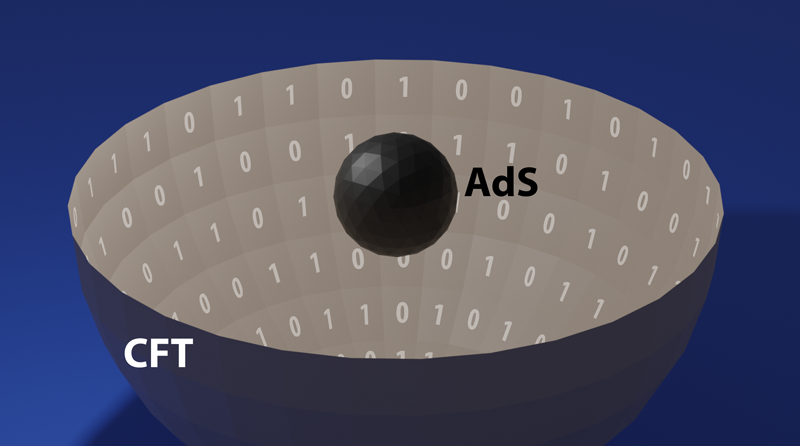
\includegraphics[width=0.95\textwidth]{images/ads-cft-blackhole}    		
    	\end{center}
    	\textit{Above: AdS / CFT visual of black hole entropy}. \cite{zayasMicroscopicAccountBlack2020}
    \end{block}
\end{column}
\begin{column}{0.55\textwidth - 1cm}


%%%%%%%%%%%%%%%%%%%%%%%%%%%%%%%%%%%%%%%%%%%%%%%%%%%%%
%                 BLOCK: ABSTRACT                   %
%%%%%%%%%%%%%%%%%%%%%%%%%%%%%%%%%%%%%%%%%%%%%%%%%%%%%
    \begin{block}{Talk Abstract}
        The Anti-de Sitter/Conformal Field Theory (AdS/CFT) correspondence states that for a certain quantum system with gravity there is an equivalent field theory system without gravity.  I will review some recent developments within the AdS/CFT correspondence where the Bekenstein-Hawking entropy of certain black holes has been given a microscopic, statistical mechanical foundation in terms of partition functions of the dual field theories. At the quantum level, the entropy of black holes is not exactly equal to one quarter of the area of the event horizon; it receives tiny quantum corrections proportional to the logarithm of the area. I will describe how these logarithmic corrections to the black hole entropy can be computed and how to match them successfully to a microscopic description based on the AdS/CFT correspondence.  
    \end{block}


%%%%%%%%%%%%%%%%%%%%%%%%%%%%%%%%%%%%%%%%%%%%%%%%%%%%%
%                BLOCK: BACKGROUND                  %
%%%%%%%%%%%%%%%%%%%%%%%%%%%%%%%%%%%%%%%%%%%%%%%%%%%%%
    \begin{block}{Brief Background}
        The second law of thermodynamics requires that black holes (BHs) have entropy. Typically, entropy scales with the volume of the region in which micro-states live. However, BHs forbid access to states in the interior. The Bekenstein-Hawking entropy scales with the area of the horizon of the BH (depicted below). \cite{baggioliGravityHolographyApplications}

         \begin{columns}
        	\begin{column}{.5\linewidth}
            	\begin{center}
		    		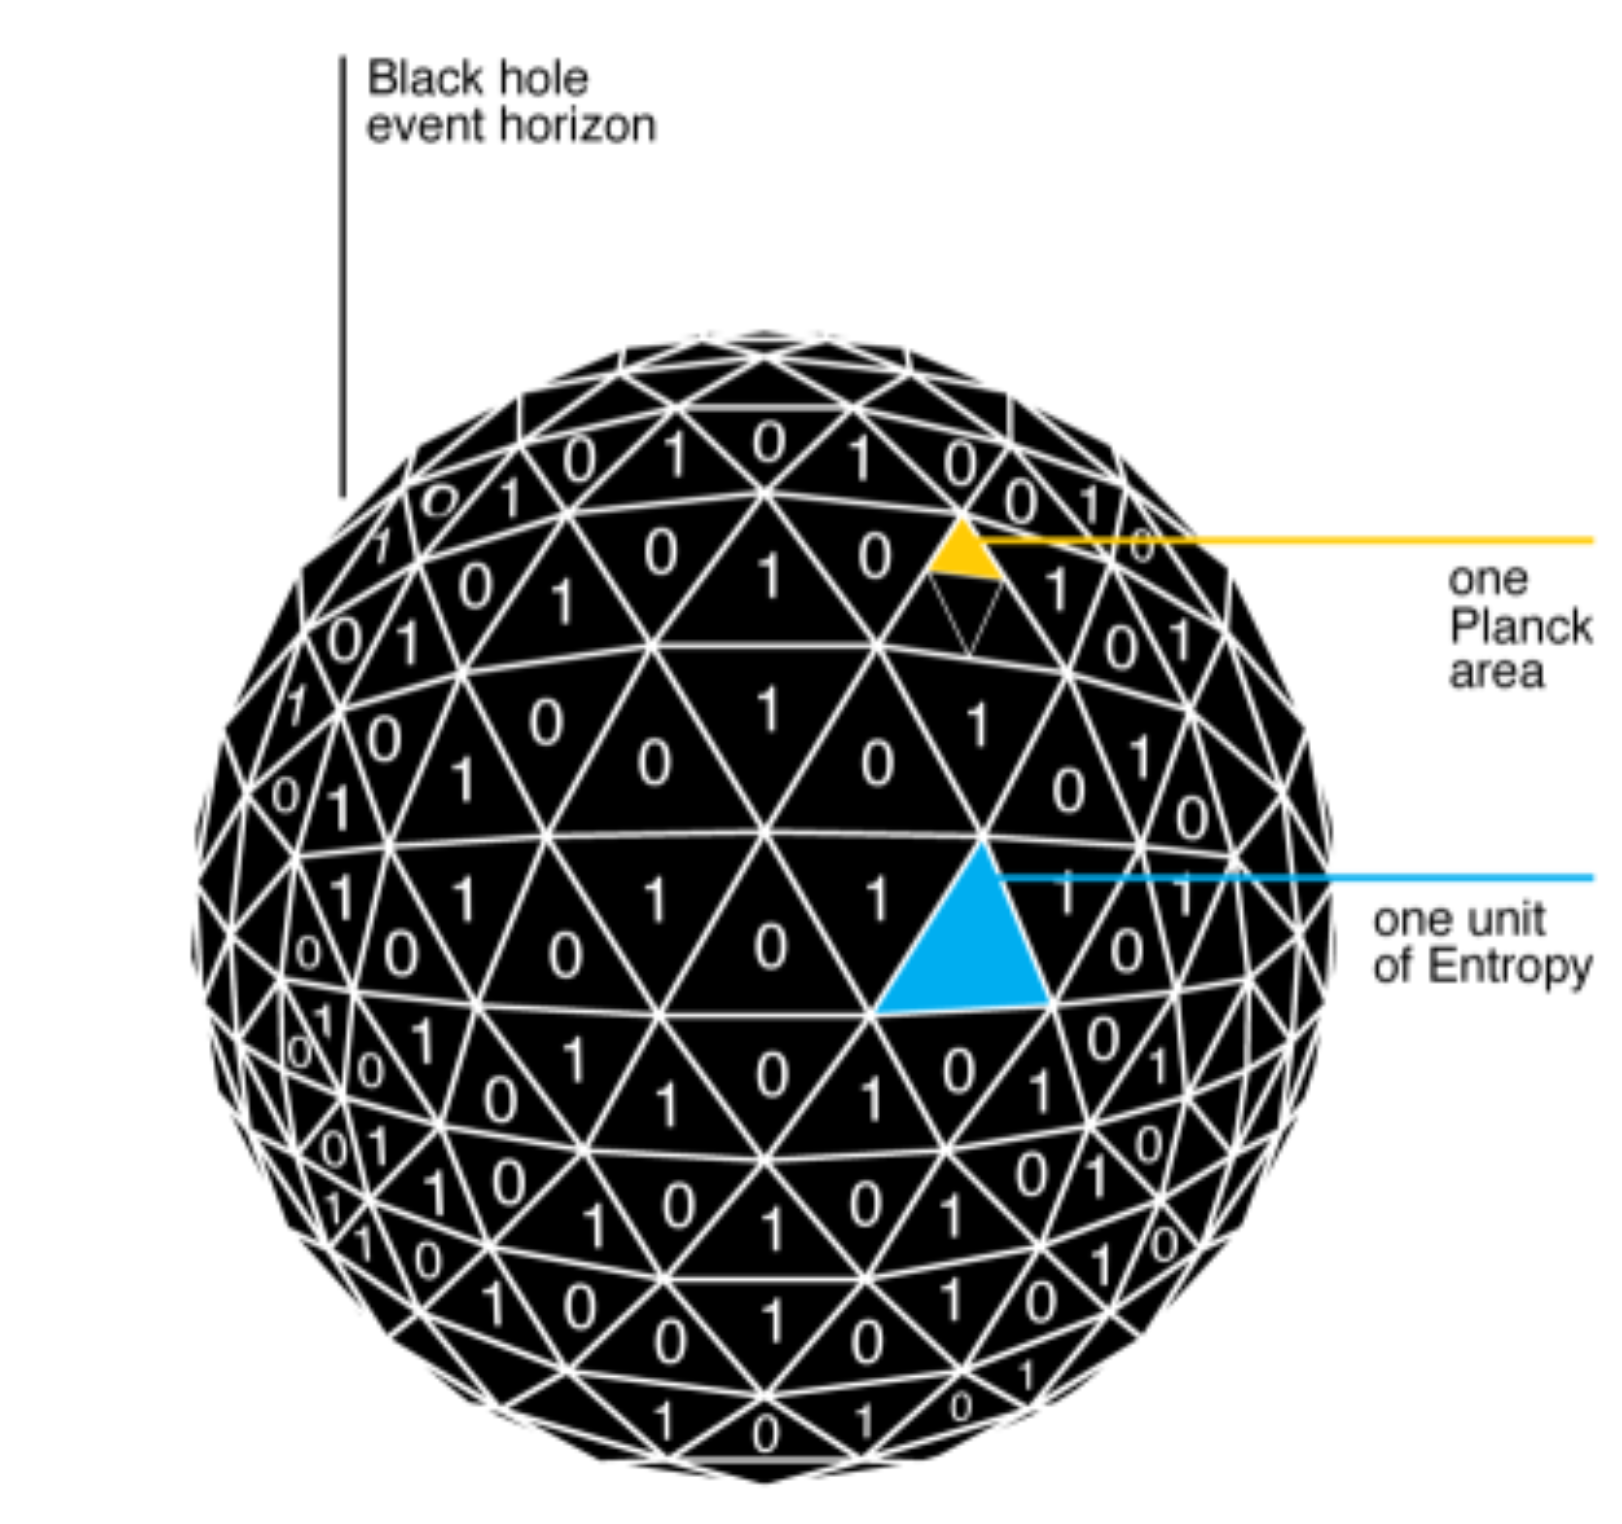
\includegraphics[width=0.85\textwidth]{images/bekenstein-hawking-entropy}    		
    			\end{center}
    	    \end{column}
        	\begin{column}{.5\linewidth}
        		\vspace{5cm}
            	$$\HUGE{S_{BH} = \frac{A}{4L_p^2}}$$ 
            	
            	$$A=16 \pi (GM/c^2)^2$$
            	
            	$$(\text{Schwarzschild})$$
    	    \end{column}
	    \end{columns}
	    \vspace{1cm}
        
    	That a $d$-dimensional conformal field theory (CFT) lives on the “boundary” of a $(d + 1)$-dimensional asymptotic Anti-de-Sitter (AdS) space can be seen as an explicit realization of the holographic principle. Using AdS/CFT correspondence, entropy counting was demonstrated for a class of five-dimensional extremal black holes, which provided a statistical interpretation of Bekenstein Hawking entropy. \cite{stromingerMicroscopicOriginBekensteinHawking1996} The ability to count states in CFT and map between AdS/CFT could provide a concrete way of counting the microstates of the BH and resolve the standing question of whether the Bekenstein-Hawking entropy counts all or only some of the microstates of the black hole. \cite{zayasMicroscopicAccountBlack2020}

    \end{block}


%%%%%%%%%%%%%%%%%%%%%%%%%%%%%%%%%%%%%%%%%%%%%%%%%%%%%
%                 BLOCK: REFERENCES                 %
%%%%%%%%%%%%%%%%%%%%%%%%%%%%%%%%%%%%%%%%%%%%%%%%%%%%%
    \begin{block}{References}
        \bibliographystyle{aipnum4-1}
		\bibliography{references}
    \end{block}

\end{column}
\end{columns}


%%%%%%%%%%%%%%%%%%%%%%%%%%%%%%%%%%%%%%%%%%%%%%%%%%%%%
%                    FOOTER TEXT                    %
%%%%%%%%%%%%%%%%%%%%%%%%%%%%%%%%%%%%%%%%%%%%%%%%%%%%%
\begin{textblock}{0.5}(0.18, 0.94)
    \color{white}
    \sffamily
    \textbf{Eberly College of Science}
    \\
    Department of Physics
\end{textblock}


%%%%%%%%%%%%%%%%%%%%%%%%%%%%%%%%%%%%%%%%%%%%%%%%%%%%%
%                   END TEMPLATE                    %
%%%%%%%%%%%%%%%%%%%%%%%%%%%%%%%%%%%%%%%%%%%%%%%%%%%%%
\end{frame}
\end{document}
